\documentclass[11pt]{article}

\usepackage{outlines}
\usepackage{graphicx}
\usepackage[T1]{fontenc}
\usepackage{subcaption}
\usepackage[margin=1in]{geometry}

\usepackage{geometry}
\usepackage[square,sort,comma,numbers,super]{natbib}
\usepackage{pdflscape}
\usepackage[colorlinks,allcolors=blue]{hyperref}
\usepackage{afterpage}

\usepackage[utf8]{inputenc}
\usepackage{xcolor}
\definecolor{textblue}{rgb}{.2,.2,.7}
\definecolor{textred}{rgb}{0.54,0,0}
\definecolor{textgreen}{rgb}{0,0.43,0}

\usepackage{enumitem}
\setlist{nosep}

\usepackage{listings}
\usepackage[export]{adjustbox}
\usepackage{wrapfig}



\lstset{language=Java, 
lineskip=-.1cm,
stepnumber=1,
numbersep=2pt, 
tabsize=4,
basicstyle=\ttfamily,
keywordstyle=\color{textblue},
commentstyle=\color{textred},   
stringstyle=\color{textgreen},
frame=none,                    
columns=fullflexible,
keepspaces=true,
xleftmargin=\parindent,
showstringspaces=false}

\graphicspath{ {./images/} }

\setlength{\parindent}{0pt}

% pt = project title; shorthand
\newcommand{\pt}{Multi-User Poker Game}
\newcommand{\pn}{Rekop}

\title{Dissertation Report: \pt}
\author{James Scully}

\setcounter{tocdepth}{4}
\setcounter{secnumdepth}{5}



\begin{document}

{\fontfamily{cmss}\selectfont}



\newcommand{\cardheight}{6em}

\newcommand{\tenclubs}{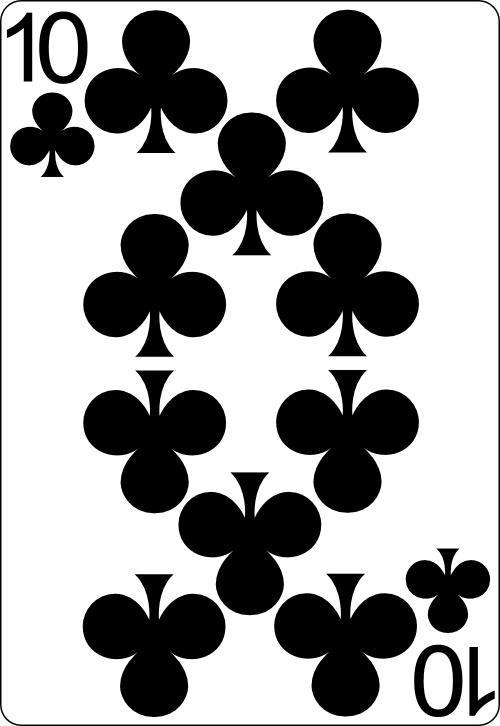
\includegraphics[height=\cardheight]{cards/10_of_clubs.png}}
\newcommand{\tendiamonds}{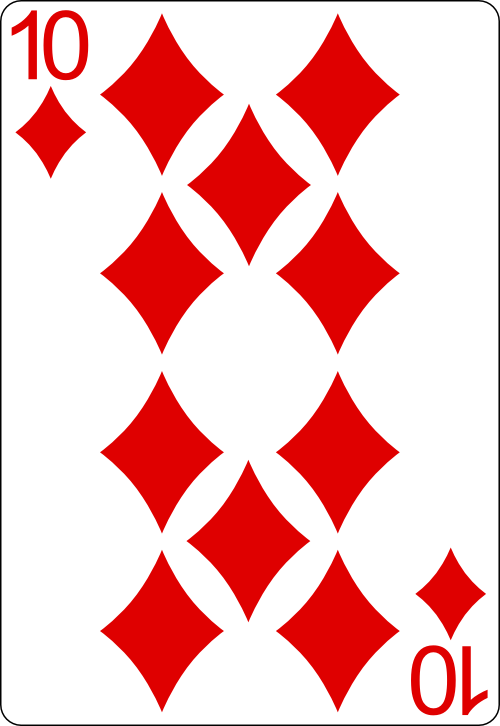
\includegraphics[height=\cardheight]{cards/10_of_diamonds.png}}
\newcommand{\tenhearts}{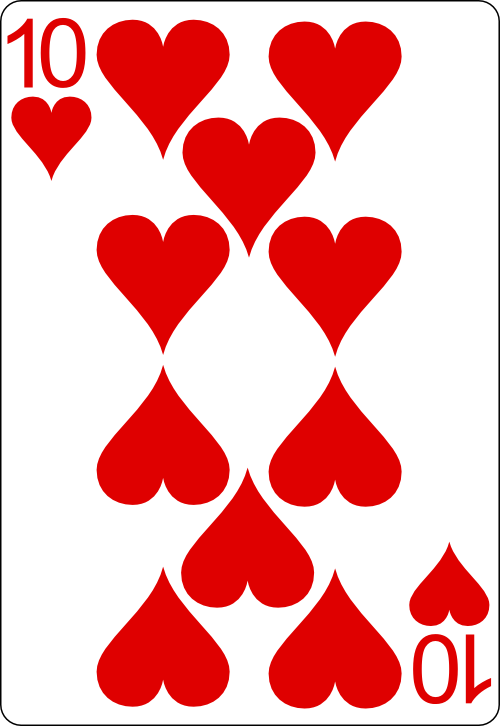
\includegraphics[height=\cardheight]{cards/10_of_hearts.png}}
\newcommand{\tenspades}{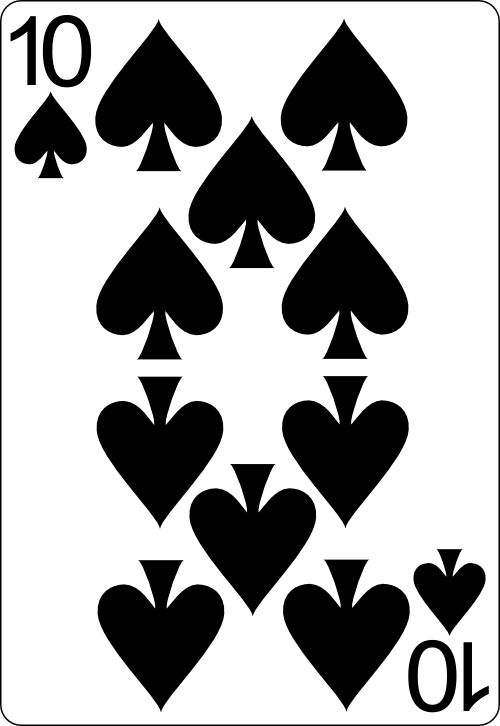
\includegraphics[height=\cardheight]{cards/10_of_spades.png}}
\newcommand{\twoclubs}{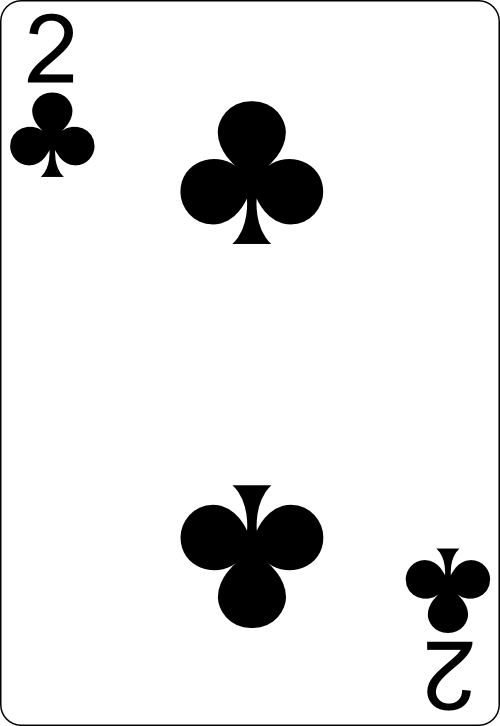
\includegraphics[height=\cardheight]{cards/2_of_clubs.png}}
\newcommand{\twodiamonds}{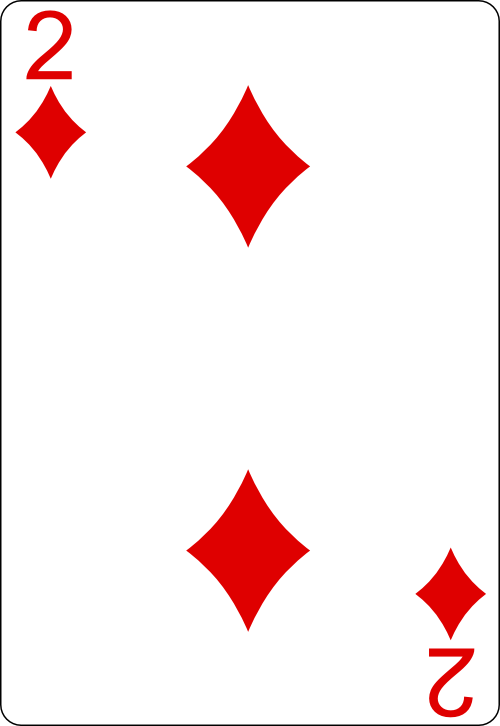
\includegraphics[height=\cardheight]{cards/2_of_diamonds.png}}
\newcommand{\twohearts}{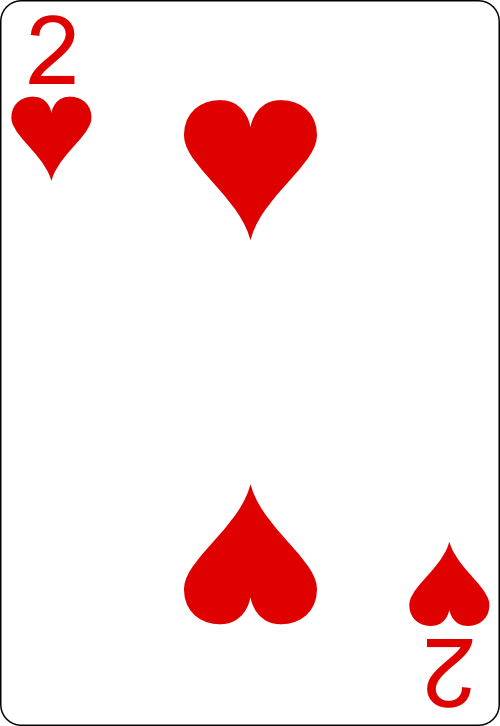
\includegraphics[height=\cardheight]{cards/2_of_hearts.png}}
\newcommand{\twospades}{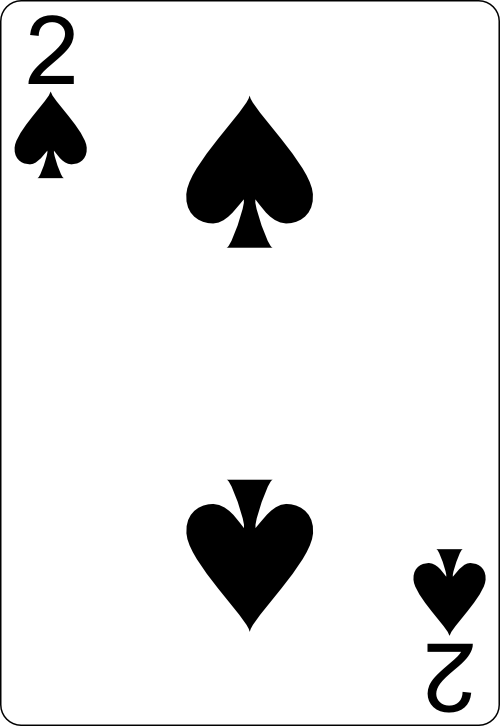
\includegraphics[height=\cardheight]{cards/2_of_spades.png}}
\newcommand{\threeclubs}{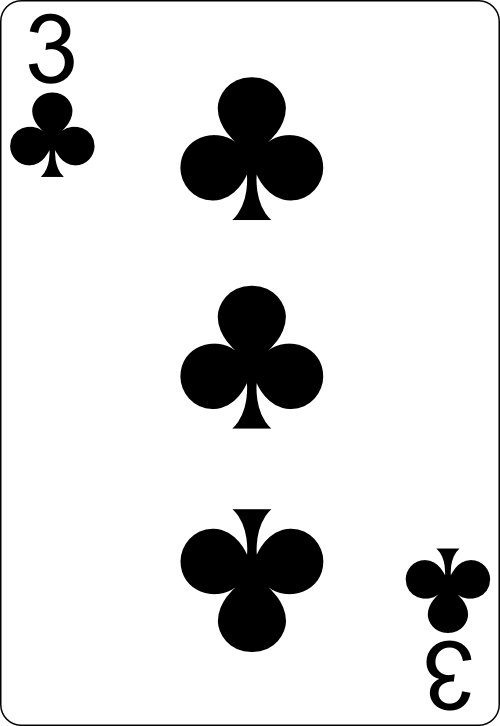
\includegraphics[height=\cardheight]{cards/3_of_clubs.png}}
\newcommand{\threediamonds}{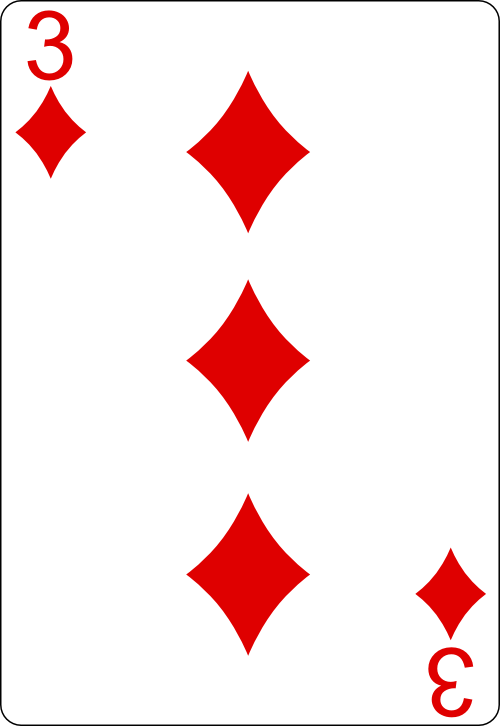
\includegraphics[height=\cardheight]{cards/3_of_diamonds.png}}
\newcommand{\threehearts}{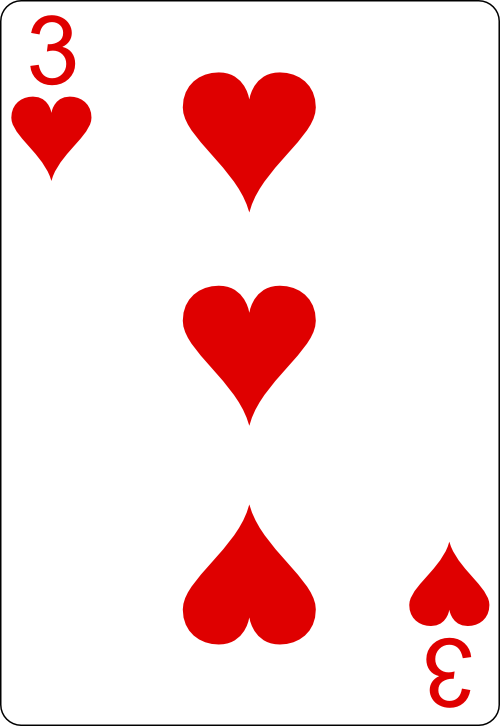
\includegraphics[height=\cardheight]{cards/3_of_hearts.png}}
\newcommand{\threespades}{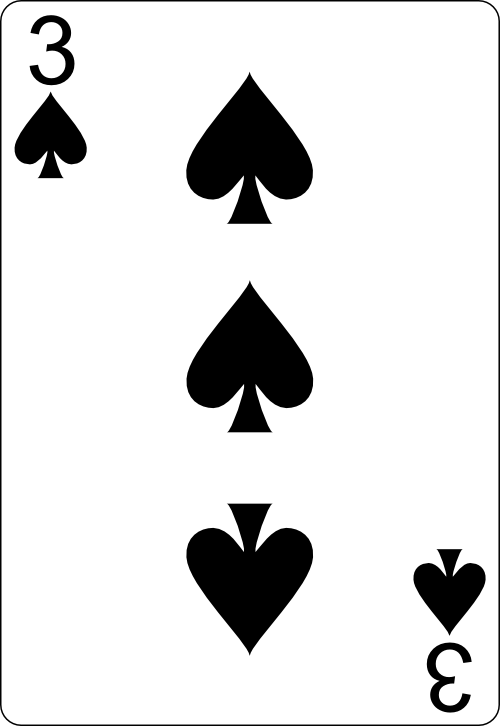
\includegraphics[height=\cardheight]{cards/3_of_spades.png}}
\newcommand{\fourclubs}{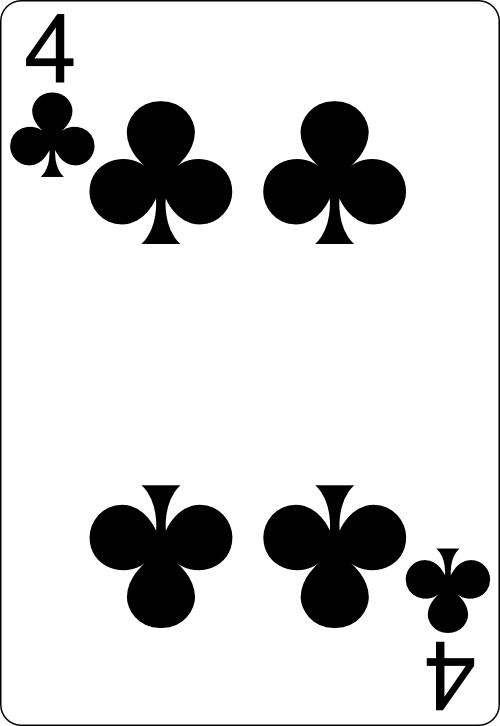
\includegraphics[height=\cardheight]{cards/4_of_clubs.png}}
\newcommand{\fourdiamonds}{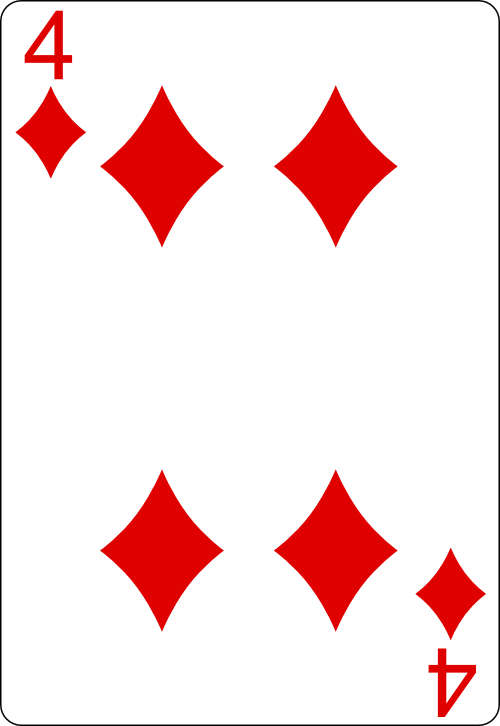
\includegraphics[height=\cardheight]{cards/4_of_diamonds.png}}
\newcommand{\fourhearts}{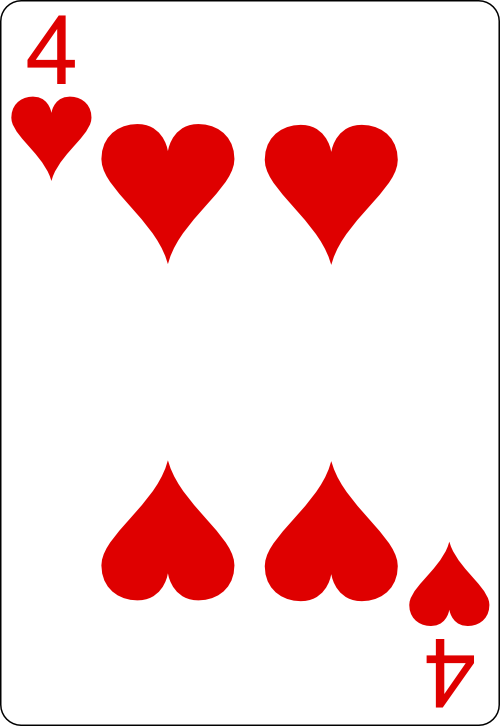
\includegraphics[height=\cardheight]{cards/4_of_hearts.png}}
\newcommand{\fourspades}{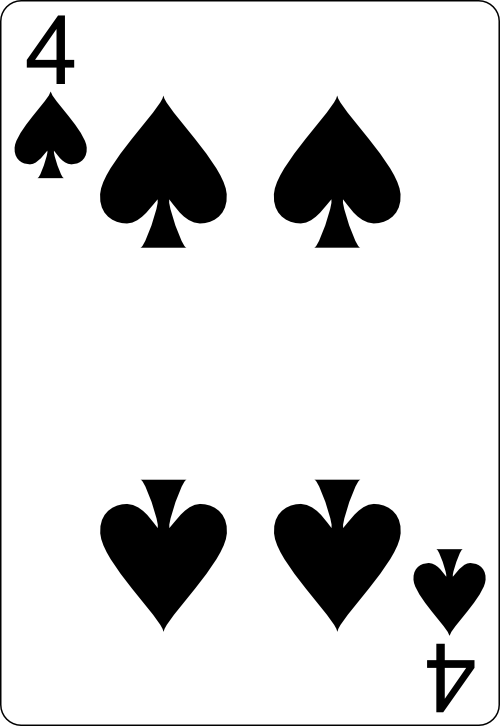
\includegraphics[height=\cardheight]{cards/4_of_spades.png}}
\newcommand{\fiveclubs}{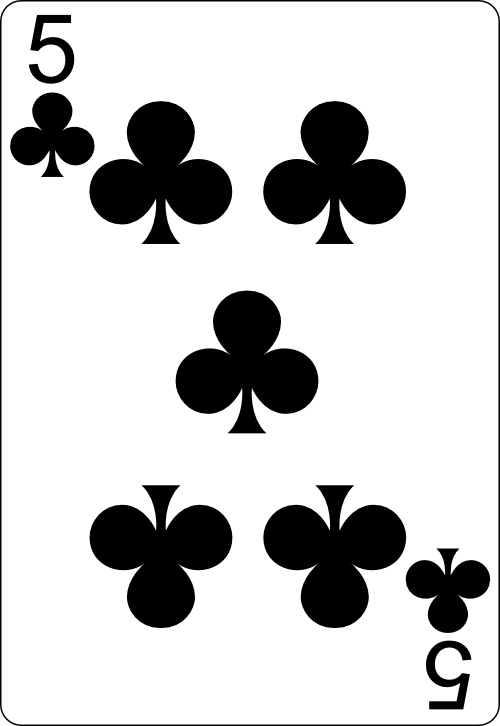
\includegraphics[height=\cardheight]{cards/5_of_clubs.png}}
\newcommand{\fivediamonds}{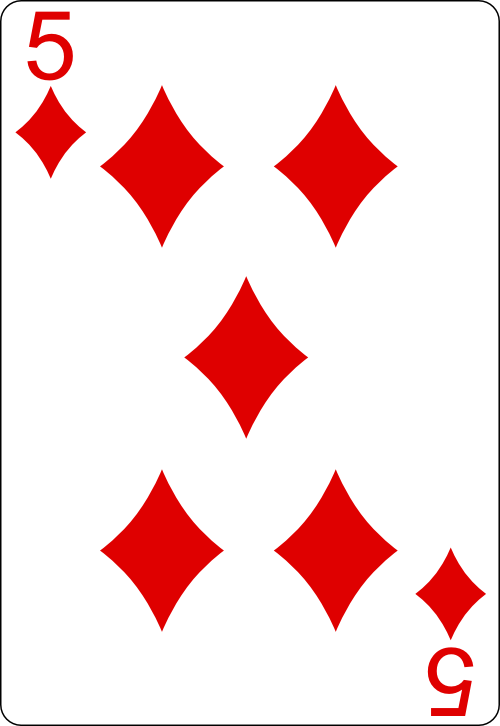
\includegraphics[height=\cardheight]{cards/5_of_diamonds.png}}
\newcommand{\fivehearts}{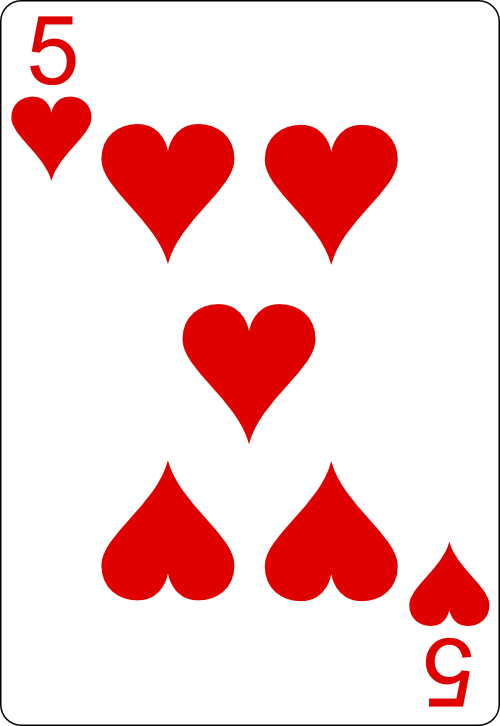
\includegraphics[height=\cardheight]{cards/5_of_hearts.png}}
\newcommand{\fivespades}{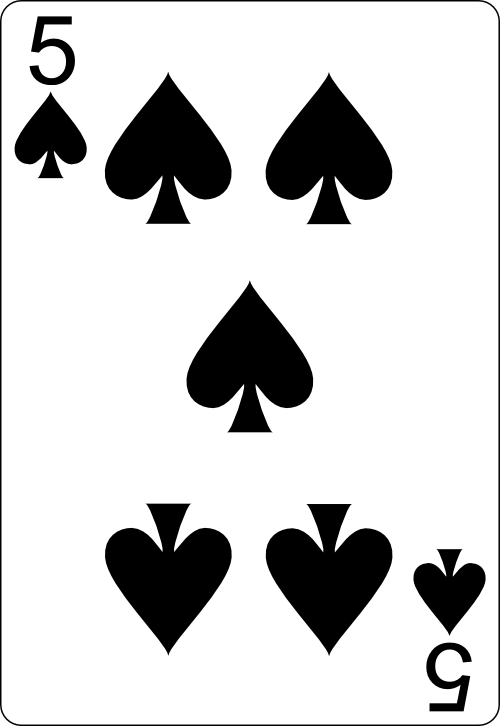
\includegraphics[height=\cardheight]{cards/5_of_spades.png}}
\newcommand{\sixclubs}{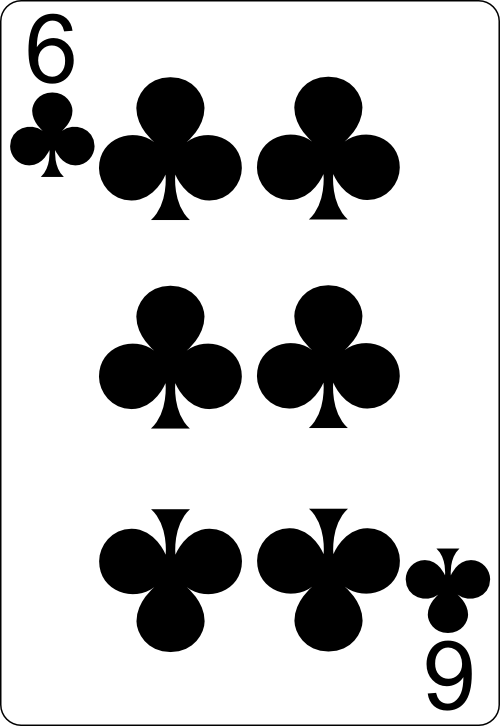
\includegraphics[height=\cardheight]{cards/6_of_clubs.png}}
\newcommand{\sixdiamonds}{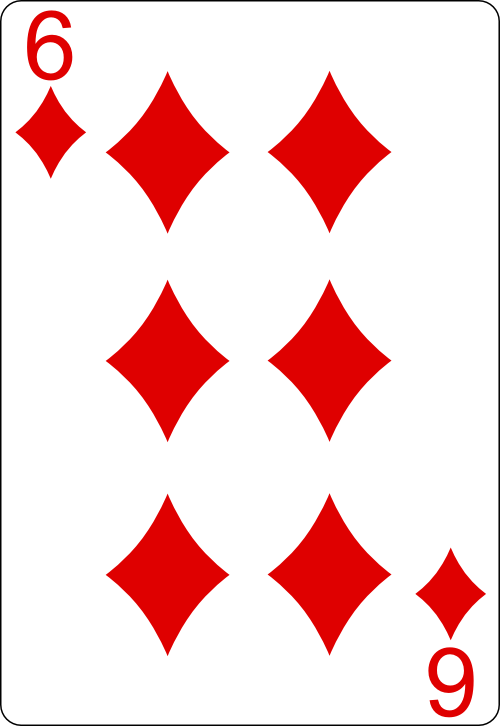
\includegraphics[height=\cardheight]{cards/6_of_diamonds.png}}
\newcommand{\sixhearts}{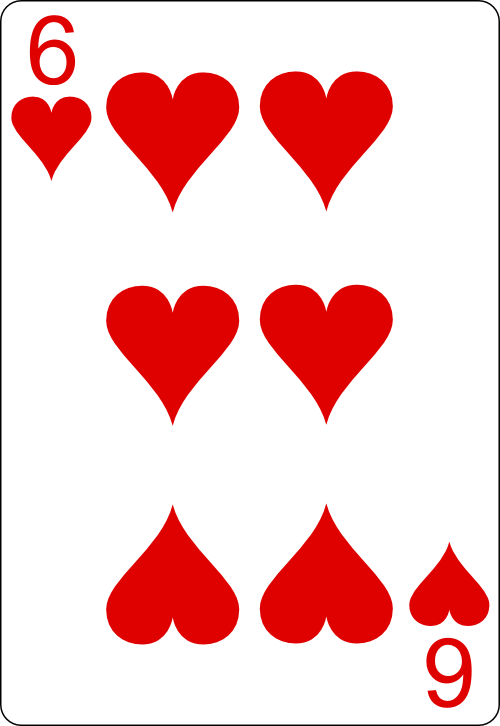
\includegraphics[height=\cardheight]{cards/6_of_hearts.png}}
\newcommand{\sixspades}{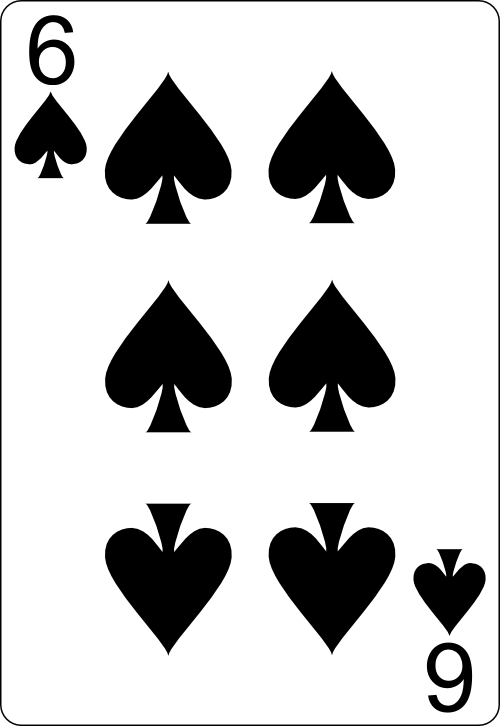
\includegraphics[height=\cardheight]{cards/6_of_spades.png}}
\newcommand{\sevenclubs}{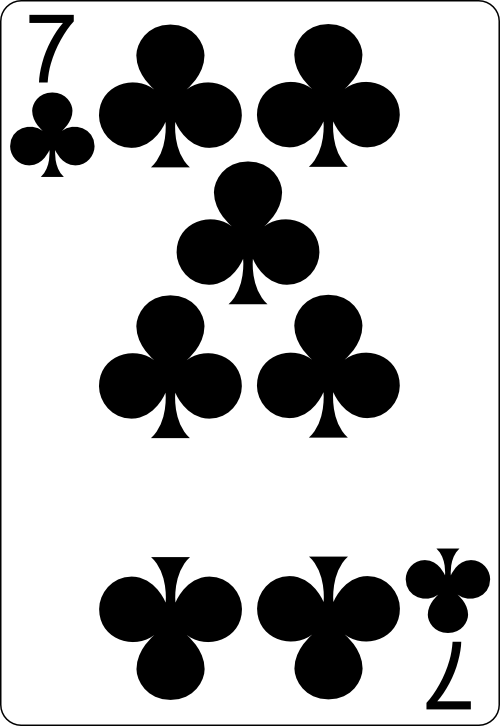
\includegraphics[height=\cardheight]{cards/7_of_clubs.png}}
\newcommand{\sevendiamonds}{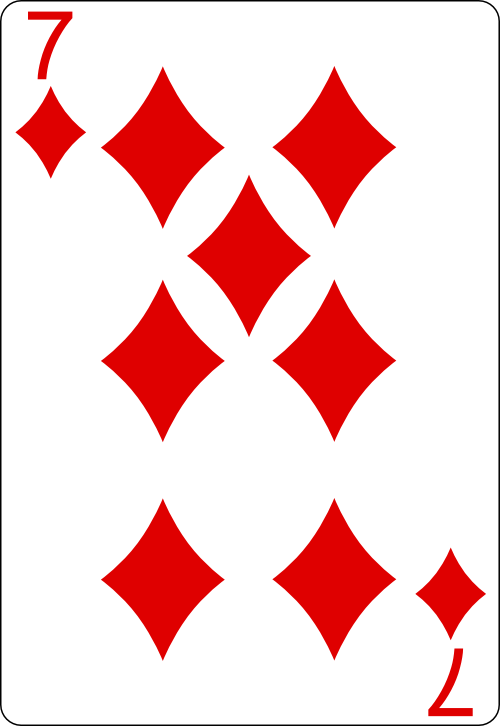
\includegraphics[height=\cardheight]{cards/7_of_diamonds.png}}
\newcommand{\sevenhearts}{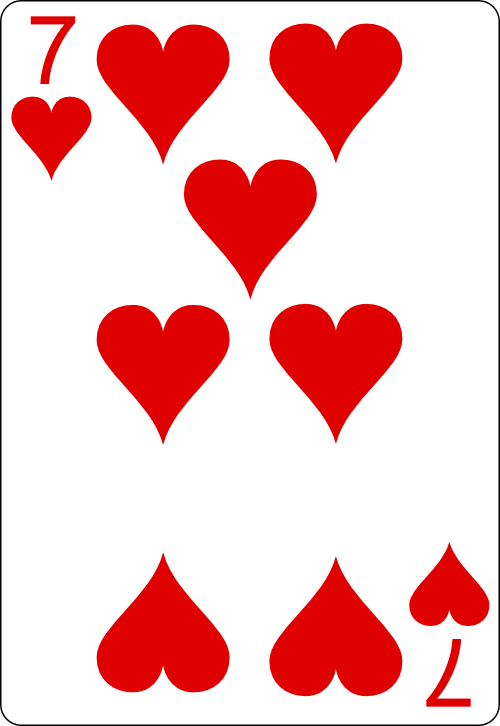
\includegraphics[height=\cardheight]{cards/7_of_hearts.png}}
\newcommand{\sevenspades}{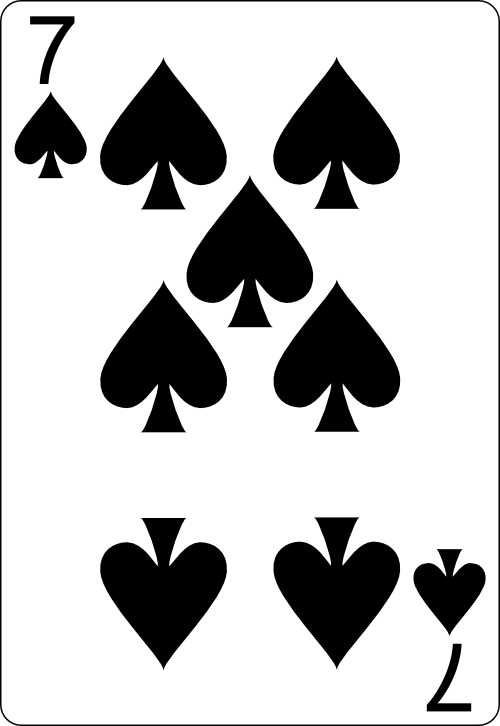
\includegraphics[height=\cardheight]{cards/7_of_spades.png}}
\newcommand{\eightclubs}{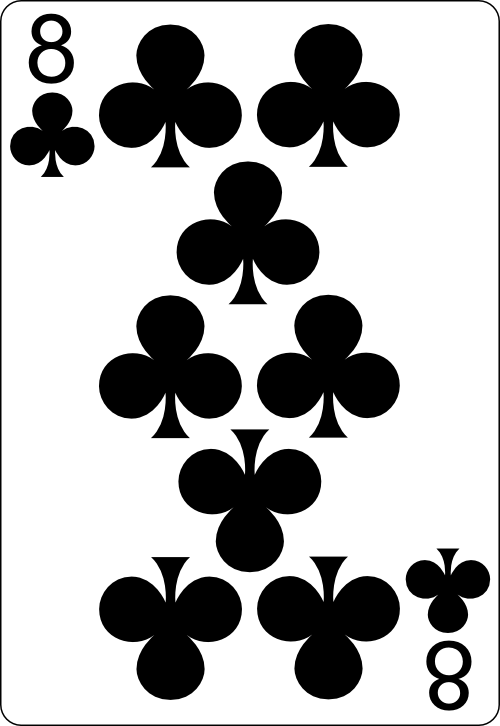
\includegraphics[height=\cardheight]{cards/8_of_clubs.png}}
\newcommand{\eightdiamonds}{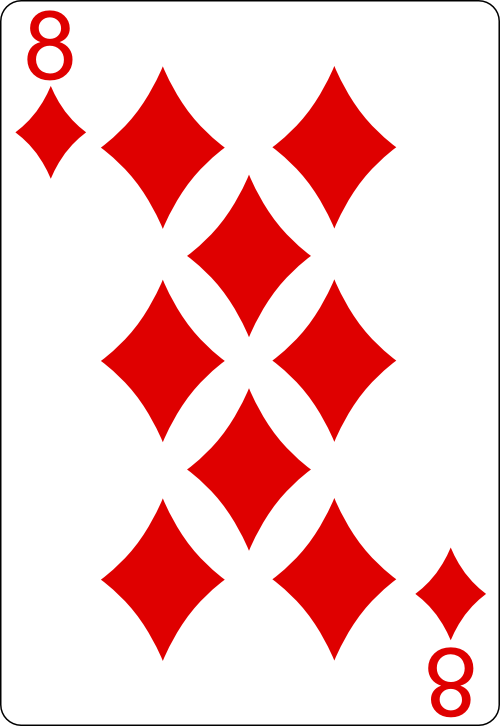
\includegraphics[height=\cardheight]{cards/8_of_diamonds.png}}
\newcommand{\eighthearts}{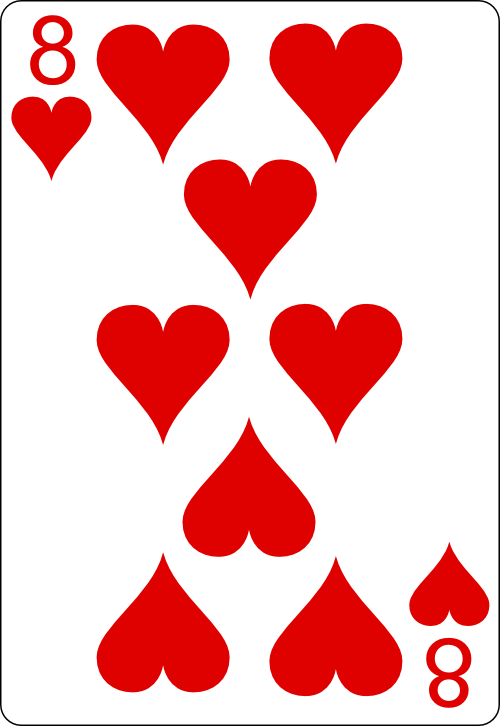
\includegraphics[height=\cardheight]{cards/8_of_hearts.png}}
\newcommand{\eightspades}{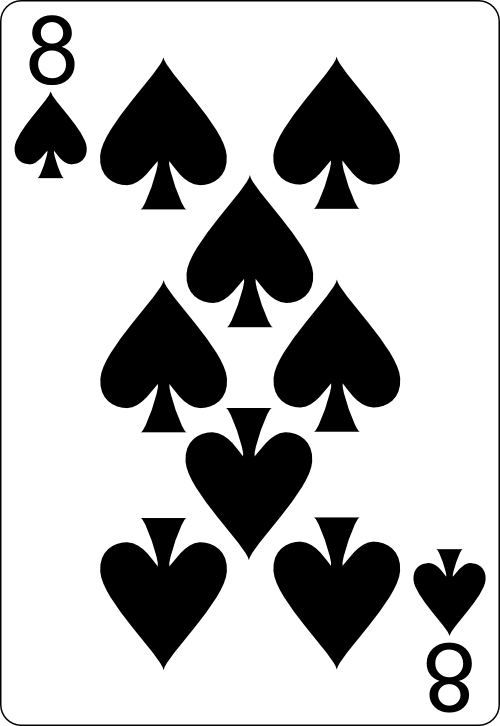
\includegraphics[height=\cardheight]{cards/8_of_spades.png}}
\newcommand{\nineclubs}{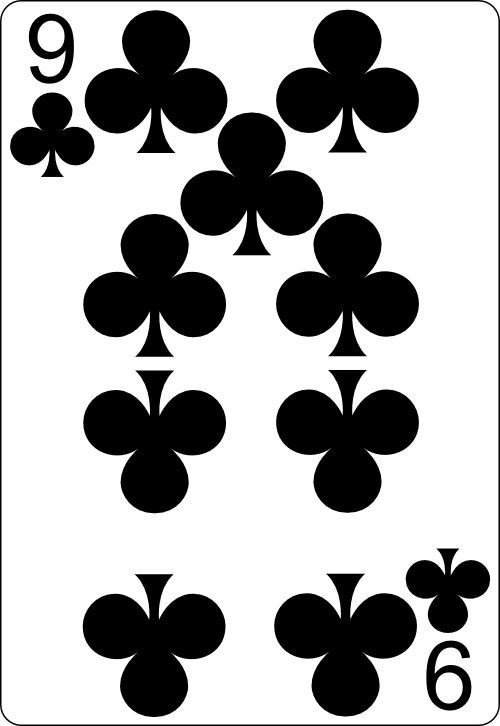
\includegraphics[height=\cardheight]{cards/9_of_clubs.png}}
\newcommand{\ninediamonds}{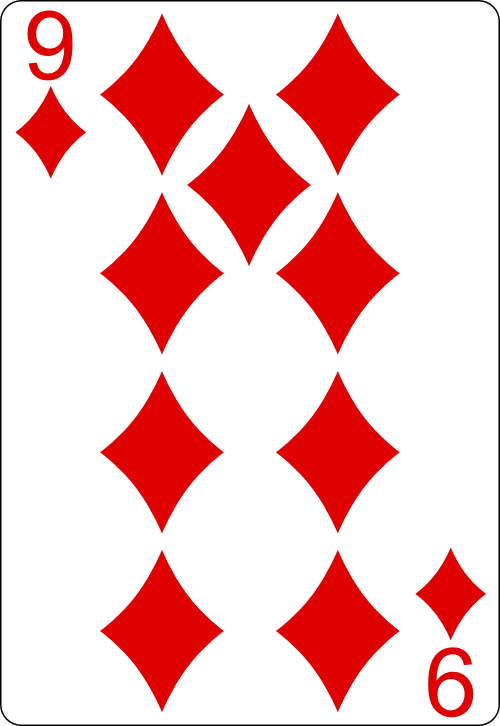
\includegraphics[height=\cardheight]{cards/9_of_diamonds.png}}
\newcommand{\ninehearts}{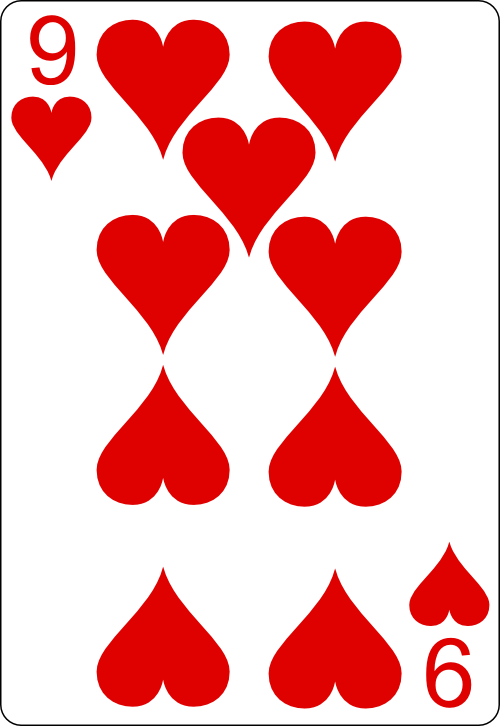
\includegraphics[height=\cardheight]{cards/9_of_hearts.png}}
\newcommand{\ninespades}{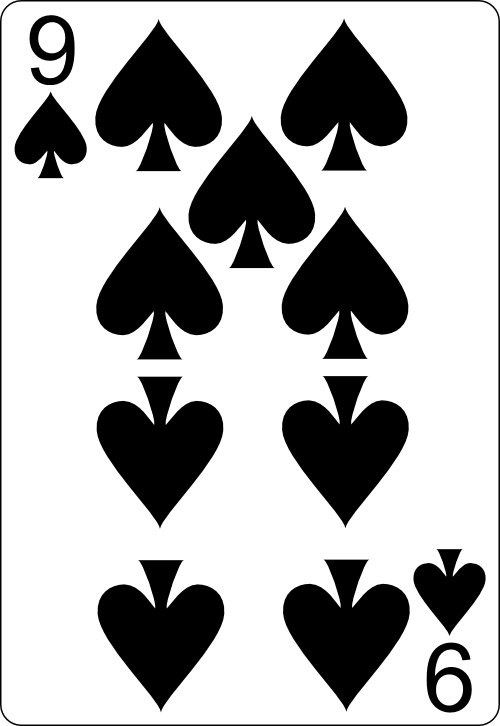
\includegraphics[height=\cardheight]{cards/9_of_spades.png}}
\newcommand{\aceclubs}{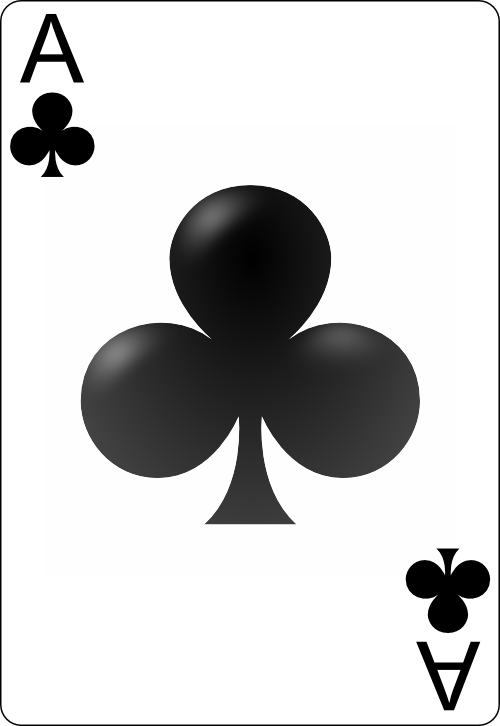
\includegraphics[height=\cardheight]{cards/ace_of_clubs.png}}
\newcommand{\acediamonds}{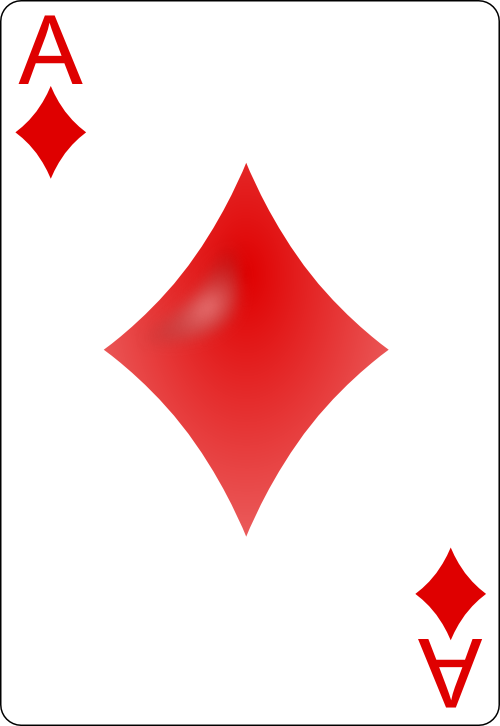
\includegraphics[height=\cardheight]{cards/ace_of_diamonds.png}}
\newcommand{\acehearts}{
\includegraphics[height=\cardheight]{cards/ace_of_hearts.png}}
\newcommand{\acespades}{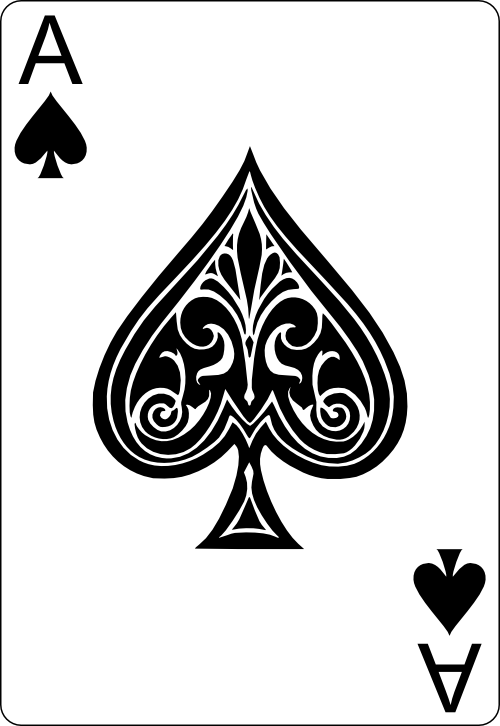
\includegraphics[height=\cardheight]{cards/ace_of_spades.png}}
\newcommand{\jackclubs}{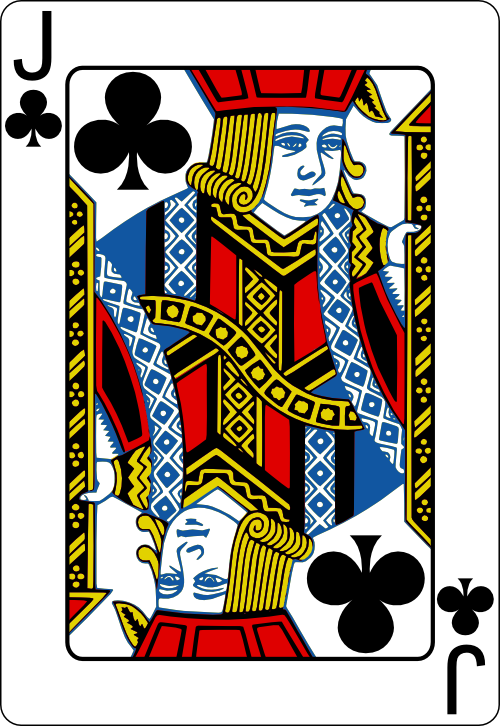
\includegraphics[height=\cardheight]{cards/jack_of_clubs.png}}
\newcommand{\jackdiamonds}{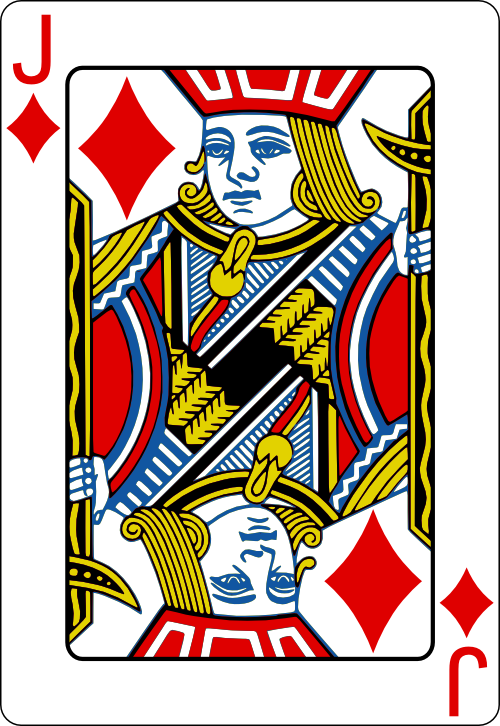
\includegraphics[height=\cardheight]{cards/jack_of_diamonds.png}}
\newcommand{\jackhearts}{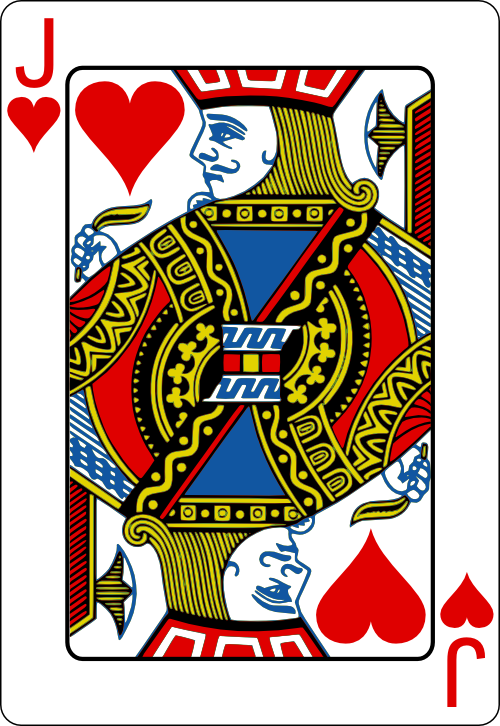
\includegraphics[height=\cardheight]{cards/jack_of_hearts.png}}
\newcommand{\jackspades}{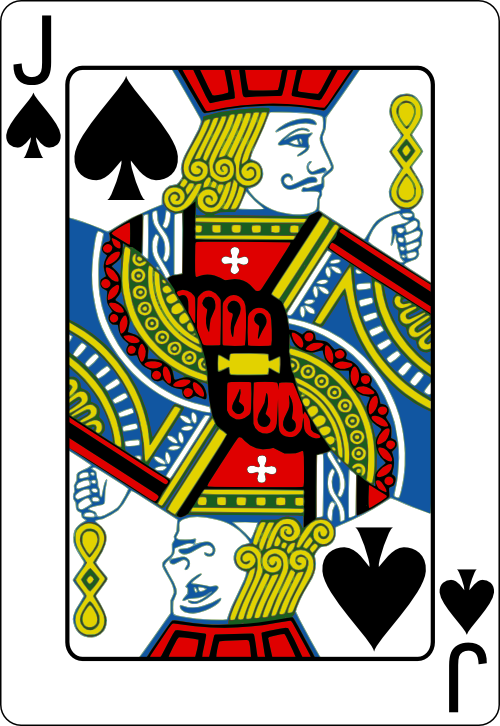
\includegraphics[height=\cardheight]{cards/jack_of_spades.png}}
\newcommand{\kingclubs}{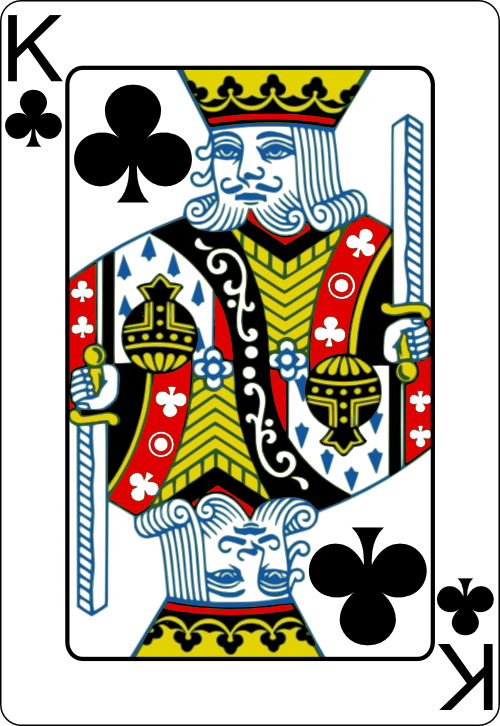
\includegraphics[height=\cardheight]{cards/king_of_clubs.png}}
\newcommand{\kingdiamonds}{
\includegraphics[height=\cardheight]{cards/king_of_diamonds.png}}
\newcommand{\kinghearts}{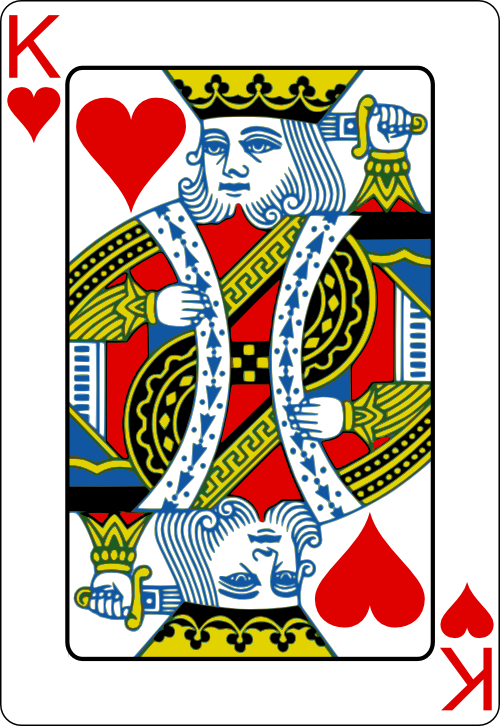
\includegraphics[height=\cardheight]{cards/king_of_hearts.png}}
\newcommand{\kingspades}{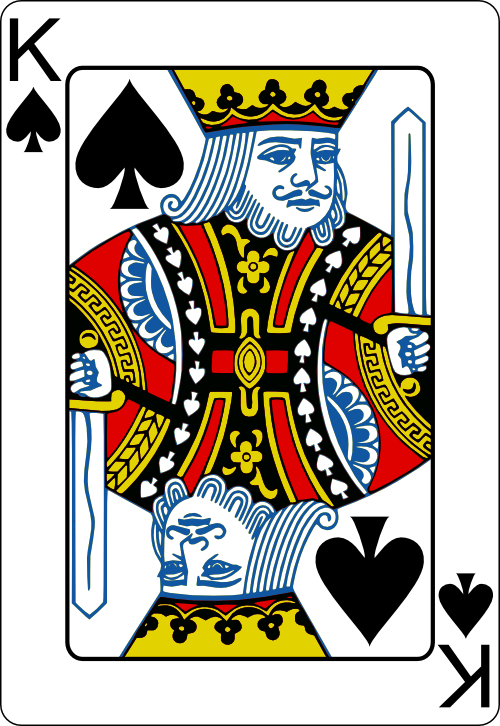
\includegraphics[height=\cardheight]{cards/king_of_spades.png}}
\newcommand{\queenclubs}{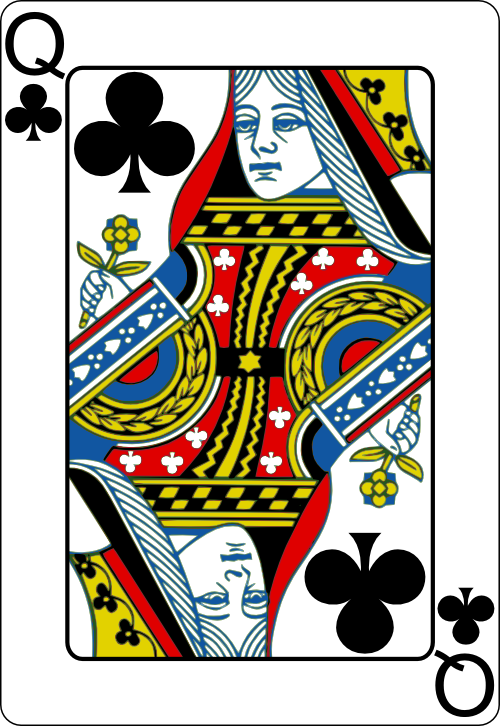
\includegraphics[height=\cardheight]{cards/queen_of_clubs.png}}
\newcommand{\queendiamonds}{
\includegraphics[height=\cardheight]{cards/queen_of_diamonds.png}}
\newcommand{\queenhearts}{\includegraphics[height=\cardheight]{cards/queen_of_hearts.png}}
\newcommand{\queenspades}{\includegraphics[height=\cardheight]{cards/queen_of_spades.png}}




\hspace{0pt}

\vfill

\begin{center}
	\includegraphics[scale=0.4]{uni_logo}
	
	\vspace{1cm}
	
	{\Large \textbf{Dissertation Report} 
		\linebreak
		Multi-user Poker Game with Disconnection Tolerance: 		
		\linebreak

		\textit{Rekop Poker}} 		
		\linebreak
		

	\textbf{I hereby declare that this dissertation is all my own work, except as indicated in the text}\\
	\textbf{Signature}: J. W. Scully \\
	\textbf{Date}: 13/12/2019 \linebreak
		
	\begin{large}
		James Scully (14304469) \\
		psyjs20@nottingham.ac.uk \\
		G400 Computer Science \linebreak \\ 
	\end{large}
	
\end{center}

\vfill

\begin{center}
	\textbf{Project Supervisor:} Milena Radenkovic
\end{center}

\hspace{0pt}

\pagebreak


\newcommand{\entry}[1]{
	\textbf{#1} - 
}

\newcommand{\TODO}[1]{
	\textbf{{\Large \emph{#1}}}
}



\tableofcontents



\newpage


%%%
% Page 1: 
%%%

\section{Introduction}


	
Poker is a type of card game that is played and watched in tournaments by many around the world. Because of it's wide popularity, it has spawned multiple types, the most popular one being Texas Hold'em, which is the main type used in both research \hyperlink{research_texas}{(A Gilpin, 2006)} and is the main variant used in the World Series of Poker \hyperlink{wsop_texas}{(WSOP, 2019)}. Other types include the similar yet lesser-known Omaha hold'em and Five-card draw; a simpler type of poker, which does not utilize the typical table seen in both hold'ems. \\

When one looks for a casual poker game that offers power to the actual end user, rather than attempting to fish money it can be quite difficult to find. From the authors own personal experience and observations with free and open software, it can be quite difficult to implement in some areas (such as games), however the ability to control a game how you would like and the ability to not have to rely on companies servers, trudge through in-application payments and ads is a unseen experience today. Some also do not allow for players with unreliable connections to continue; they are simply dropped from the game.  \\

I believe that many of these are far too focused on the financial aspect of the game and neglect the small groups whom simply would like another medium to play poker. This is because lobbies are often not customizable and will drop players whom do not have a good enough network connection to the lobby, so that more players are able to join.  \\

To remedy these issues, Rekop poker will be developed to handle disconnections or unstable connections by reserving their place in the lobby and the ability to join back when the player is available to. It will also not feature micro-transactions and provide the ability for players to host their own servers, with their own settings.

\section{Motivation}
Rekop poker aims to provide a new, alternative to other multi-player applications on the Google Play store, as many of these prevent user customization and introduce in-application purchases, with no ability for players to play locally on their own network. 

It is for this reason that Rekop poker is being developed, so that there is an open-source alternative where players have the control over the game as opposed to company owned servers and incentives to make money. 

\newpage
\section{Methodology}

Test-Driven Development has been essential so far in the development of the poker algorithm. Evaluating Texas Hold'em hands has many vectors of errors and being able to write tests before and alongside implementation helped out immensely. 

Take this snippet from the testing whether a hand is a straight or not: 

\begin{lstlisting}*[language=java,numbers=none]
assertTrue(new TexasEvaluator("0D 0D 2D KD AD QD JD").isStraight());
assertTrue(new TexasEvaluator("AD KD QD JD 0D QD JD").isStraight());
/* Falses */ 
assertFalse(new TexasEvaluator("0D 0D 0D 0D AD QD JD").isStraight());
assertFalse(new TexasEvaluator("2D 5D 9D JD 0D QD JD").isStraight());

\end{lstlisting}

This allowed me to rapidly create test cases, but more importantly easily generate cases which could break the method itself via edge cases or worst case scenarios. For example, one issue that was resolved was the method would register duplicate cards as being a straight, i.e. only 4 sequential cards would be needed. \\

Agile has also been a driving development cycle - primarily creating a very basic yet functional version of the software and accepting of changing requirements. For example, the back-end was created first so that the game mode itself was in an acceptable state. From here, it made it easier to visualize how the server would handle sending, receiving and processing the player's cards. \\

Though this helps develop a certain sector and thus the entire project succeed, as observed by the link of Agile/iterative incentive to success in \hyperlink{agile_success}{(P Serrador, 2015)}, it can lead to over-development of one area and cause tunnel-vision, as was the case with not developing both the poker back-end and the server software at-least somewhat concurrently. For a time-constrained project like this, it is best to find a middle-ground.


\newpage
\section{Design}

\subsection{Overview}

The project itself is being broken down into three compartments - a backend that satisfies the core Texas Hold'em gamemode, the server which will provide the connections needed for players to play together on their own networks and the Android application, which links both of these together with the graphical interface. \\

The system as a whole is very server-sided, as this holds all the data instead of the clients. Appendix 7.3 shows the basic design of the system, whereby the client only receives its current hand, the ranking of their hand and the cards currently shown on the table. \\

For this project, we'll be developing on Android with use of standard Java libraries, though this is subject to change. Artwork will be designed with myself, with the addition of royalty-free music as needed. This will be credited. 

\subsection{Backend}

The backend is written solely in Java as the language itself is platform agnostic - Android being reliant upon Java (bytecode). This also allows for the server to run on Linux, Windows and Mac, as per the requirements. It has been broken down in such a way that game modes other than Texas Hold'em can be added to it, enabling further development down the line. \\

For example, we've created data classes for Faces and Suits, each containing values for easy comparison. Furthermore, we've created a Deck class that allows for the user to pull a random card from a standard 52-card deck and ensure that it hasn't been pulled before. These building blocks allow for future development by providing the basics needed in a standard card game.


\newpage

\subsection{Networking}
\subsubsection{Introduction}
The networking is based upon client-server architecture using a Thread-pool written in Java. Initially, we wished to use a Peer-to-Peer / UPnP approach, however disconnection-tolerance, whilst possible, can become extremely difficult to implement; given that all clients would have to be constantly synchronized on the state of the host, then delegate a host if the original was to disconnect. %c 

\subsubsection{Thread-pool}
In any case where a server must have multiple clients connected, it is ideal that each client holds an individual thread. This allows for each thread to execute a task on its own, or the server to choose a thread to act upon. %c %may have to add diagram

The threads on the server are not used as a handler to the server, whereby the client passes/receives messages to and from the server. Instead, the server program itself handles data flow, by assigning and keeping track of each input/output (I/O) stream when a client connects. We encapsulate the thread within a Player object, which holds the IO streams, the players chips, ID and other statistics used. \\

This approach was taken as code complexity would have increased, as we would un-necessarily have a middle-man in the connection. For example, Client A passes that they've decided to raise their bet by 500. This would then be passed to the thread through it's own input stream. Then, the thread would output this action through it's output stream to the servers input stream.

Another notable reason it was chosen to simply pass over one IO stream is that the Java implementation of IO streams is quite fragile; they must only be declared once, with the output stream being declared before the input. 

In more varying programs, such as the likes of computer games, where the user is more 'free' in their actions i.e. they are not limited to three actions (call/raise/fold), this approach would be more appropriate. %c



\subsubsection{Client}

The client program does not contain much processing, it is left up to the server to decide whether their input is valid. This primarily comes from initial development of the backend, where it was simple text messages send between the client and the server. Since the implementation in the Android application is simple button presses, the user input cannot be invalid since all decisions are set in concrete. \\


\subsubsection{Communication / Diagram}






%\subsection{Server}
%
%Initially, an idea as defined in our Vision and Scope document was to use a UPnP / Peer to Peer approach, however this is infeasible as a key requirement of this project is disconnection-tolerance. This is because if the host is to lose connection permanently or temporarily, the rest would be unable to play.
%
%This is where we've opted for a client-server approach; as this allows atleast for one solid host, separate from the clients whom are likely to suffer connection issues. \\
%
%The servers design is such that on the start of the game, the server knows exactly what cards are going to be placed on the actual table, i.e. the initial flop (3 cards), turn and river albeit these will not be released to the player until necessary. It is responsible to send what cards each player has, and will utilize the previously mentioned Deck object to deal hands out. \\
%
%Therefore, the only messages required by the client to send are their actions, such as how much they are betting, whether they fold or raise. We are still investigating into how we can transform this to allow for disconnection tolerance.

%\begin{center}
%\includegraphics[scale=0.65]{server_diag}
%\end{center}

\newpage
\subsection{User Interface / Android application}

The most critical part and the binding element of this project is the actual mobile application itself. The user interface is to be kept simple, with the main menu being a simple strip of buttons that can be added to for extra gamemodes or features. There is a navigation bar that will allow the user to switch between playing, statistics, profile and to exit. 
The interface is required to be simple, as this allows for intuitive and good user experience with the application. \\

The following figure shows how we've changed our initial wireframe slightly. As we've implemented it into Android, we've attempted to make it appeal to certain conventions, such as using the Hamburger icon for the menu and moving it to the side of the screen.

\begin{figure}[h]
	\makebox[\textwidth][c]{
	\begin{subfigure}[h]{0.5\textwidth}
		\includegraphics[width=\textwidth]{menuwireframe}
		\caption{Wireframe}
	\end{subfigure}	
	
	\begin{subfigure}[h]{0.6\textwidth}
		\includegraphics[width=\textwidth]{menuapp}
		\caption{Android sketch}
	\end{subfigure}	
	}
	
	\caption{A slightly altered production of wireframe}
	
\end{figure}

\begin{figure}[h]
\makebox[\textwidth][c]{
	\includegraphics[width=\textwidth]{poker_table}
	}
	\caption{Android sketch of playing a match}
	
\end{figure} 

\newpage


\subsection{Algorithms}

\entry{Hand Strength}
The algorithm for hand-strength is very basic and as such is inefficient, however this is not the main focus of the project. The base of our algorithm is in a TexasEvaluator class, whereby we test each potential result i.e. straight, flush in their own methods. We then sequentially run these methods in order of ranking, so that we can return a result. \\


\entry{Win evaluation}
Win evaluation can be done by sorting each players hand by result, i.e. Royal Flush, Four of Kind, Straight. If each player has a unique result, then we can simply take the top result, in this case Royal Flush. If two players contest the highest result, e.g. a Straight, then we'll look at the highest card in the TResult object, which determines each players result (i.e. Three of a Kind) and the highest card. \\

If two players contest the highest result, but have the same highest card, then the pot is split as is the normal result in poker. 

\section{Implementation}

\subsection{Project Requirements}
Our requirements for the project were not particularly specific, however some core ones were defined in our vision and scope, as well as project proposal. 

\subsubsection{Backend}
\textbf{Functional}
\begin{itemize}
	\item Programmed in Java (or Kotlin)
	\item Able to generate a result (i.e. 3 of kind) from the players hand and table
	\item Abstracts elements of card-based games (i.e. hands, cards, faces)
\end{itemize}
%\textbf{Non-Functional}
%\begin{itemize}
%	
%\end{itemize}

\subsubsection{Server}
\textbf{Functional}
\begin{itemize}
	\item Runs on Linux and Windows
	\item Handles the evaluation of games internally
\end{itemize}

%\textbf{Non-Functional}
%\begin{itemize}
%
%\end{itemize}

\subsubsection{Application}

\textbf{Functional}
\begin{itemize}
	\item Runs on devices using Android KitKat and above
	\item Allows for connecting to servers via IP address
	\item Scalable interface for screens with low resolutions (1280 x 720)
\end{itemize}

\textbf{Non-Functional}
\begin{itemize}
	\item Presents a simple, uncluttered interface for connecting/joining games
	\item Presents a simple game screen, with not too much clutter for game statistics
	\item Presents the users current chips for online matches
	\item Presents the users current chips within the game
	\item Presents a server browser for online matches
\end{itemize}

\newpage



\subsection{Client}
\subsubsection{Overview}
Our initial idea for the client was to develop it as solely as an Android application. However, as we'll discuss, this made testing very difficult to do. 

\begin{itemize}

\end{itemize}

\subsubsection{Design}
The client is written in Java for compatibility with the Android ecosystem, and also the server itself. However, it was designed such that it is not a mobile application itself but rather an interface for the application to use. This was because during development, it made unit testing the client much easier as it was ran locally on the machine. Beyond this, the author's home network was restricted, meaning that running the client and server on the same machine meant they could connect, and multiple instances of the client could be run. 

In order to develop disconnection tolerance, we required that the server had some method of identifying what clients had connected and an anonymous token was generally the best way to go about this. During design, we investigated multiple avenues for this, including the server taking note of the connecting clients MAC addresses and storing them. 

This wasn't suitable however, as the Java method of getting MAC addresses is difficult and not easily comparable. Another was to use the username of the client connecting, but this would lead to conflicts if another person with the same name was to join - the originally disconnected player wouldn't be allowed back in. 

Instead, we decided to opt for an identity file approach, whereby upon installing the application the user has a generated key file that when connecting to servers, send a unique identifier. This way, conflicts do not occur (very unlikely, with a 32-character identifier being generated).







\subsubsection{Development}






\subsection{Server}
\subsubsection{Overview}
As the target of disconnection tolerance implies, the server was a crucial part of the project. It also however took a lot of effort to coordinate with the client, as any changes made to the client would need to be synchronized with the server, and so development of both had to be done somewhat in parallel. 

We had multiple challenges to overcome when developing the server, including:

\begin{itemize}
	\item Allowing multiple clients to connect
	\item Gracefully deal with disconnections
	\item Allow only those who'd previously lost connection back
	\item Find a suitable method for hosting the server
\end{itemize}

\subsubsection{Design}
For the server, we needed a way for each connection to exist independent of each other, meaning that if one was to disconnect, the others would not experience issues because of this. Because a single-threaded server meant that only one client could be served at a time, we settled on a thread-pool approach. This meant that in the case a connection was to disconnect, we can remove the thread from the pool and move to the next, viable client. 

%!% add figure to support

When a player disconnects either on purpose or unexpectedly, 









\subsubsection{Development}








The server at this moment in time is very basic and barebones - it only operates on String messages passed back between the server and the client thread and has not yet fully implemented the Texas Hold'em gamemode. \\

\begin{wrapfigure}{r}{0.5\textwidth}
\includegraphics[width=0.9\linewidth]{server_workings} 
\caption{Current and future workings of inner server}
\label{fig:wrapfig}
\end{wrapfigure}

It operates upon a thread-pool, where we can have multiple connections on their own thread, allowing for multiple tasks - in this case, connections - to be processed \hyperlink{threadpool}{(Oracle, 2019)}.  \\


Figure 2 shows how the inner workings of the server is speculated to work. Each thread within the pool will communicate with a database or other medium of storage, as this allows for each action to be recorded.\\



So far, we can communicate between the client and each thread for certain actions, however the next step is to coordinate these requests between, as shown in the figure, a centralized database/storage medium, so that we can pass all actions to our backend evaluator. \\

Figure 3 shows our bi-directional communication between the client connection and its parent thread. Note that though these are simply text messages currently this is the foundation for future development, whereby we can execute necessary code on requests.

Appendix entries 7.5 and 7.6 show our methods currently for both our TPokerThread and TPokerClient.


\begin{figure}[h]
	\makebox[\textwidth][c]{
	\begin{subfigure}[h]{0.6\textwidth}
		\includegraphics[width=\textwidth]{demo_server}
		\caption{Server receiving data from clients}
	\end{subfigure}	
	
	\begin{subfigure}[h]{0.6\textwidth}
		\includegraphics[width=\textwidth]{demo_client}
		\caption{Client showing received enums and card, sending commands}
	\end{subfigure}	
	}
	
	\caption{Demonstration of bidirectional server-client communication}
	
\end{figure}

\newpage

\subsection{Face}
For the Face, we opted to use an enumerated type (enums) as these are generic datatypes that are both easy to read in code (they do not need to be initialized each time) and can be assigned values similar to normal classes.  \\

This was chosen because it simplifies reading the code, but they can also easily define other values in their constructor. Enums can easily be transferred over a network via their value name or id. The code following shows this, as we can set a custom display value, e.g. "Three" and a value for the card. Later on, we can use these values to sort hands and make determining straights and other results much easier. 

\begin{lstlisting}*[language=java,firstnumber=0]
public enum Face {

	// these can be accessed as Face.TWO, Face.ACE, etc. 
    TWO   ("Two", 0),
    THREE ("Three", 1),
    FOUR  ("Four", 2),
    FIVE  ("Five", 3),
	...
    JACK  ("Jack", 9),
    QUEEN ("Queen", 10),
    KING  ("King", 11),
    ACE   ("Ace", 12);

    private final int val;
    private final String str;

    Face(String display, int value) {
        this.str = display;
        this.val = value;
    }
}
\end{lstlisting}

\newpage
\subsection{Evaluating Hands of Texas Hold'em}

I decided it was best to have multiple methods for evaluating a hands rank as other methods of implementing this involved lookup tables or other more convoluted methods, such as representing cards as 52-bit numbers and performing bitwise operations on them. Though lookup tables are very quick to evaluate \hyperlink{lookup}{(L. Teofilo, 2013)}, I felt that for this project having clear and handwritten code was more suitable as this project is marked upon my own work. It also is much easier to read than bit-wise operations or complex lookup-table generation. \\

The evaluate method itself contains the following code: 

\begin{lstlisting}*[language=java]
    public TResult evaluate() {
        // these conditions must be done in sequence, for order of rankings
        TResult kindOutput = getKinds();
        // this is required so that StraightFlushFlag is set
        TResult isStraight = isStraight();
        // variable to hold each test
        TResult result = null;
        // assignment in if statement is to remove calling method twice
        if( (result = isRoyalFlush()) != null)
            return result;
        if(StraightFlushFlag)
            return isStraight;
        // because kindOutput may be null, we need to ignore it to get past to straight
        try {
            if(kindOutput.rank == Rank.FOUR_OF_KIND)
                return kindOutput;
            if(kindOutput.rank == Rank.FULL_HOUSE)
                return kindOutput;
        } catch (NullPointerException ignored) { }
        if( (result = isFlush()) != null)
            return result;
        if(isStraight != null)
            return isStraight;
        if(kindOutput != null)
            return kindOutput;
        // the highest card will always be first as we use a sorted collection
        return new TResult(cards.get(0).face, Rank.HIGH_CARD);
    }
\end{lstlisting}


\newpage
\subsection{Determining a Straight}
Determining whether a hand is a straight would be difficult had we not assigned values to the Face values of our cards. Take the following table, whereby the first two cards are the players, the other 5 are on the table. \\

\begin{center}
\tendiamonds \twoclubs \ \ \ \ \ \ \  \eightclubs \ninehearts \sixdiamonds \fiveclubs \sevenspades
\end{center}

This hand's highest rank would be a straight, as we 10 - 5 in the hand; though they are not displayed as in order. \\

Take for example we start off with the first card, 10 of Diamonds. We would have to find any card on the table that is either a Jack or a 9. From here, we would then have to branch off and see if there is a card that is a Queen or an Eight, for either direction. This would have to be done for each card on the table, and optimizations would make the code more complex and introduce more areas where bugs or incorrect results can slip in.\\

However, since we have assigned each of the Faces values as seen previously in Section 5.2 we can use Java's Collections library to sort our cards from highest to lowest. This way, we only need to search in one direction, i.e. if the next card is lower than our current one; which is shown in Appendix 7.4. This will reduce code complexity and also the worst case scenario; we don't have to arbitrarily search the entire deck for an 'adjacent' number.


\newpage
\section{Progress}
\subsection{Management}
To help me manage what needs to be done in the project and primarily drive development, GitLab issues tracker have been made for various tasks that need to be completed. These are easy to read via the use of labels and offer reminders through school email. In addition to this, branches are created for each issue to manage changes to code.  \\

In the initial design stages, I focused on the vision and scope whereby outlining the ideal product but also the bare essentials for the project. Working under agile principles, I focused on getting a usable algorithm for evaluating poker hands as this gives us early ideas from where to go next or problems that would arise; once we had this to a good state, research for how the server will handle sending these objects or communicating became easier.  \\

Appendix 7.1 and 7.2 show the old and the new Gantt charts. Upon developing the backend, I realised that no databases and thus database classes were needed in this part. Later on during the end stages of the servers development, databases will be used for online play, and can be removed at this stage. Therefore, server tasks aswell as implementing them into the Android application have been brought forward, as these are critical.  \\

\subsection{Contributions and Reflections}

A key goal of all software is that it must be efficient - both in terms of code complexity and performance. Upon undertaking this project it was naively assumed that, given how easy it is to recognize the outcome of a poker round in reality, it wouldn't be too difficult to implement efficiently through code. \\

It is therefore that the algorithm currently used is very compartmentalized, and potentially slower than some implementations (such as look-up tables or doing bit-wise operations). For example, it takes between 50 - 100ms for one result to be calculated on a desktop computer. Since most servers will be running on one, it doesn't particularly matter about the performance as much as the other aspects of the program.\\

\newpage

Reflecting upon how I assumed Test-Driven Development would take much of our time before and during up and that we did not have "too much time to write tests and develop a fully-functional program", this proved to be false. Having instant feedback on whether it passed, what the result was and the ability to debug into it was essential. \\



Although, initially I was under the assumption that each test case was going to have to be made up of newly created objects. Test cases wrote this way were lengthy and becoming a nuisance to write. Instead, I created a factory-esque pattern within the evaluator class itself to resolve, for example, "0D 0D 2D KD AD QD JD" into a testable hand of cards.  \\

The example below shows how writing test cases becomes much easier through this method, rather than creating a new object for each test case.

\begin{minipage}{.5\textwidth}

\begin{lstlisting}
TexasHand FLUSH_FOK = new TexasHand(
    new Card(Suit.CLUBS, Face.FOUR),
    new Card(Suit.CLUBS, Face.FOUR),
    new Card(Suit.CLUBS, Face.FOUR),
    new Card(Suit.CLUBS, Face.FOUR),
    new Card(Suit.CLUBS, Face.ACE)
);
...
public void isFlush() {
    assertTrue(FLUSH_FOK.isFlush());
\end{lstlisting}
\end{minipage}
\begin{minipage}{.5\textwidth}

\begin{lstlisting}[breaklines=true]
assertTrue(new TexasEvaluator("4C 4C 4C 4C AC QS JC").isFlush());
\end{lstlisting}
\end{minipage} \\

\subsection*{Conclusion}

Currently, I am satisfied with the backend of the project as the main area of concern for this area was accuracy in determining the outcome of a game. The use of unit tests has taught me how to effectively break a problem down into small, testable blocks of code and then re-construct them into an algorithm. \\


However, I think that one area to work on would be time management and consequently gauging how much time tasks will take and overlooking key parts of this project; in particular the next step which is the server. This next step is not so easy to debug as it is not as easy as sequencing certain blocks of code together to create a system and most certainly not easy to debug. Therefore, I have pushed these tasks to the front of jobs to be done and allowed myself more time for these, as seen in the Gantt charts in the Appendix.

\newpage

\section{Appendix}

\subsection{Old Gantt Chart}
\includegraphics[width=\textwidth]{gantt_chart}

\newpage
\subsection{New Gantt Chart}

Color chart:

Purple = completed \\
Green  = to be completed\\
Orange = moved forward\\
Red = deleted\\

\includegraphics[width=\textwidth]{modified_gantt}


\newpage
\subsection{Abstract System Design}

\includegraphics[width=\textwidth]{wholesystem}


\newpage 

\subsection{Straight method}

All cards are sorted before this and other methods in the evaluator are called.

\begin{lstlisting}
public TResult isStraight() {
	int valStreak = 0;
	int suitStreak = 0;
	int origin = 0;

	// our previous value going in should be the first in the sorted array
	// note: cards is a class member containing all cards in the evaluator, 
	// sorted high to low.
	int previousVal = cards.get(0).getValue();
	Suit previousSuit   = cards.get(0).getSuit();

	for(int i = 1; i < 7; i++)  {
		// these are the attributes of card i
		Card card   = cards.get(i);
		Suit suit   = card.getSuit();
		int  value  = card.getValue();

		// if we have a previous card of same value, just skip over.
		if(previousVal == value)
			continue;

		// if the previous card was higher than the current, then add to streak
		// else, reset counter to 0.
		if(previousVal == value + 1) {
			valStreak++;

			if(suit == previousSuit)
				suitStreak++;
			else
				suitStreak = 0;

		} else {
			valStreak = 0;
			origin = i;
		}

		// if we've already managed a straight, then return true.
		// note that this should return the highest STRAIGHT, as we're descending down.
		if(valStreak == 4) {
			// this removes the need for ANOTHER function for Strt. Flushes.
			if(suitStreak == 4)
				StraightFlushFlag = true;

			Face high = cards.get(origin).face;
			Rank result = StraightFlushFlag ? Rank.STRAIGHT_FLUSH : Rank.STRAIGHT;

			return new TResult(high, result);
		}

		previousVal = value;
		previousSuit = suit;
	}
	return null;
}
\end{lstlisting}
\newpage

\subsection{TPokerThread run method}
\begin{lstlisting}[breaklines=true]
@Override
public void run() {
	try {

		DataInputStream in  = new DataInputStream(new BufferedInputStream(client.getInputStream()));
		ObjectOutputStream out = new ObjectOutputStream(client.getOutputStream());

// concatenate data (in this case ID), face and suit as a string
		String sendData = data + " " + face + " " + suit;
		System.out.println("Sending data: " + sendData);

// write the full data string to our client's input stream.
		out.writeUTF(sendData);
		out.flush();
		
		String line = "";

// read input from the user. If we receive DISCONNECT, then we close the connection.
// else we simply print their instruction. These requests can be forwarded to other components in the future.
		while(!line.equals("DISCONNECT")) {
			try {
				line = in.readUTF();

				if(line.equals("CALL")) {
					System.out.printf("ClientID: %s has called for next round\n", data);
				} else if (line.equals("FOLD")) {
					System.out.printf("ClientID: %s has folded\n", data);
				} else if (line.split("\\s+")[0].equals("RAISE")) {
					System.out.printf("ClientID: %s has raised by: %s\n", data, line.split("\\s+")[1]);
				} else {
					System.out.printf("ClientID: %s, Message: %s\n", data, line);
				}
			} catch (IOException e) {
				System.out.println(e);
			}
		}

		// close all IO connections
		client.close(); out.close(); in.close();

	} catch (IOException e) {
		e.printStackTrace();
	}
}
\end{lstlisting}
\newpage

\subsection{TPokerClient main method}
\begin{lstlisting}[breaklines=true]
public static void main(String[] args) {
	Socket sock = null;

	DataOutputStream out = null;
	DataInputStream  in  = null;
	ObjectInputStream servOut = null;

	try {
// for now, connect to localhost (127.0.0.1) on port 1337.
// later, this will be replaced with the servers external IP address
		sock = new Socket("127.0.0.1", 1337);
		System.out.println("Connected");

		// in is our input stream, in this case command-line
		// out is the servers
		in = new DataInputStream(System.in);
		out = new DataOutputStream(sock.getOutputStream());

		// this is the connection to our TPokerThread
		servOut = new ObjectInputStream(sock.getInputStream());

		String line = (String) servOut.readUTF();

		// parse our clientID and initial card details - todo: pass two cards
		if(line == null || line.isEmpty()) {
			System.out.println("Line was null or empty");
		} else {
			System.out.println("Retrieved data (connectionID, Face, Suit): " + line);
			// re-build a Card object from Face and Suit enums
			getCardFromData(line);
		}

	} catch (IOException i) {
		System.out.println("Exception Caught");
		i.printStackTrace();
	}

	String line = "";

	// this will fail when we have a disconnect message, and close IO
	while(!line.equals("DISCONNECT")) {
		try {
			line = in.readLine();
			out.writeUTF(line);
		} catch (IOException e) { e.printStackTrace(); }
	}

	try {
		in.close(); out.close(); sock.close();
	} catch (IOException e) { e.printStackTrace(); }

}
\end{lstlisting}





\newpage
\section{Bibliography}

\renewcommand\refname{Bibliography}
\begin{thebibliography}{9}

% https://people.eecs.ku.edu/~saiedian/Teaching/Sp19/811/Papers/Agility/does-agile-work.pdf#s0055
\bibitem{agile_success}
\hypertarget{agile_success}{}
\begin{flushleft}
	Pedro Serrador, Jeffrey K. Pinto \\
	\textit{Does Agile work?—A quantitative analysis of agileproject success} \\
	Source in paragraph: \textit{4. Results} \\
	Retrieved from \url{https://people.eecs.ku.edu/~saiedian/Teaching/Sp19/811/Papers/Agility/does-agile-work.pdf#s0055}
\end{flushleft}


\bibitem{lookup}
\begin{flushleft}
\hypertarget{lookup}{}
	Luís Filipe Teófilo, Luís Paulo Reis, Henrique Lopes Cardoso \\
	\textit{Speeding-Up Poker Game Abstraction Computation: Average Rank Strength} \\
	Source in paragraph: \textit{2. Background} \\
	Retrieved from \url{https://www.aaai.org/ocs/index.php/WS/AAAIW13/paper/view/7083/6489}
\end{flushleft}

% https://www.cs.cmu.edu/~sandholm/texas_demo.aamas-06.pdf 2.1 Texas Hold'em
\bibitem{research_texas}
\begin{flushleft}
\hypertarget{research_texas}{}
	Andrew Gilpin, Tuomas Sandholm \\
	\textit{A Texas Hold’em poker player based on automated abstraction and real-time equilibrium computation} \\
	Source in paragraph: \textit{2.1 Texas Hold'em} \\
	Retrieved from \url{https://www.cs.cmu.edu/~sandholm/texas_demo.aamas-06.pdf}
\end{flushleft}


% https://www.wsop.com/tournaments/updates/?aid=4&grid=1628&tid=17580&dayof=8298&rr=5
\bibitem{wsop_texas}
\hypertarget{wsop_texas}{}
\begin{flushleft}
	World Series of Poker \\
	\textit{Champion Wins Main Event No-Limit Hold'em} \\
	Source in paragraph (uses Texas Hold'em terminology): \textit{Claas Segebrecht Eliminated in 2nd Place} \\
	Retrieved from \url{https://www.wsop.com/tournaments/updates/?aid=4&grid=1628&tid=17580&dayof=8298&rr=5}
\end{flushleft}

\bibitem{threadpool}
\hypertarget{threadpool}{}
\begin{flushleft}
	Oracle \\
	\textit{Thread Pools Documentation} \\
	Retrieved from \url{https://docs.oracle.com/javase/tutorial/essential/concurrency/pools.html}
\end{flushleft}


\end{thebibliography}


\end{document}